%% LyX 2.3.6.1 created this file.  For more info, see http://www.lyx.org/.
%% Do not edit unless you really know what you are doing.
\documentclass[english]{article}
\usepackage[T1]{fontenc}
\usepackage[latin9]{inputenc}
\usepackage{geometry}
\geometry{verbose,tmargin=2.5cm,bmargin=2.5cm,lmargin=2.5cm,rmargin=2.5cm}
\usepackage{calc}
\usepackage{textcomp}
\usepackage{graphicx}
\usepackage{babel}
\begin{document}
{[}SPLIT\_HERE{]}
\begin{enumerate}
\item \textbf{{[}YIJC/PRELIM/9597/2019/P1/Q1{]} }

According to some researches done on children below the age of 16,
it was found that the height of a boy, measured in centimetres (cm),
should lie within the normal range with: 
\noindent \begin{center}
minimum height = 5.3 \texttimes{} Age + 71 
\par\end{center}

\noindent \begin{center}
maximum height = 6.2 \texttimes{} Age + 87 
\par\end{center}

The text file HEIGHTDATA.TXT contains 20 entries of the data in the
following format: 
\noindent \begin{center}
<Name>, <Age>, <Height> 
\par\end{center}

\subsection*{Task 1.1: }

Write program code to:
\begin{itemize}
\item read the entire contents of \texttt{HEIGHTDATA.TXT}. 
\item determine if the boy\textquoteright s height lies within the normal
range. 
\item display the contents using the format given below 
\end{itemize}
\noindent %
\begin{minipage}[t]{0.5\columnwidth}%
Example run of the program: 

\textbf{Input File: }

\texttt{Ali,6,105 }

\texttt{Bob,10,145 }

\texttt{Charlie,15,185} %
\end{minipage}%
\fbox{\begin{minipage}[t]{0.5\columnwidth}%
The output generated from the input file would be: 

\texttt{\textbf{Name ~~~Age Height Within normal range }}

\texttt{Ali ~~~~6 ~~105 ~~~Yes}

\texttt{Bob ~~~~10 ~145 ~~~Yes }

\texttt{Charlie 15 ~185 ~~~No}%
\end{minipage}}

\subsection*{Evidence 1.1: }

Your program code. \hfill{}{[}6{]}

\subsection*{Evidence 1.2: }

Screenshot of the output.\hfill{} {[}2{]}

During data entry, some of the data may have been wrongly entered
with transposition errors. In the case of Charlie\textquoteright s,
his height should have been 158 cm but was wrongly transposed and
entered as 185 cm. 

\subsection*{Task 1.2: }

Write program code to: 
\begin{itemize}
\item determine the correct height for those entries outside the normal
range. 
\item display the amended contents using the format given below. 
\end{itemize}
In cases where there are more than one possible or no possible height,
print \textquoteleft Re-enter data\textquoteright .

\noindent %
\begin{minipage}[t]{0.5\columnwidth}%
Example run of the program:

\textbf{Input File:}

\texttt{Ali,6,105}

\texttt{Bob,10,145 }

\texttt{Charlie,15,185 }

\texttt{Ethan,7,131 }

\texttt{Rick,13,415 }%
\end{minipage}%
\fbox{\begin{minipage}[t]{0.5\columnwidth}%
The output generated from the input file would be:

\texttt{\textbf{Name ~~~Age Height Corrected Height}}

\texttt{Charlie 15 ~185 ~~~158}

\texttt{Ethan ~~7 ~~131 ~~~113 }

\texttt{Rick ~~~13 ~415 ~~~Re-enter data}%
\end{minipage}}

Example run of the program: 

\subsection*{Evidence 1.3: }

Your program code. \hfill{}{[}6{]}

\subsection*{Evidence 1.4: }

Screenshot of the output. \hfill{}{[}1{]}

{[}SPLIT\_HERE{]}
\item \textbf{{[}YIJC/PRELIM/9597/2019/P1/Q2{]} }

The Oxford English Dictionary, published in 1989, contains 171,476
words. Instead of doing a linear search whenever we want to find a
word, it is more efficient to perform a binary search. 

\subsection*{Evidence 2.1: }

Describe the binary search algorithm. \hfill{}{[}2{]}

\subsection*{Task 2.1: }

Write a program \texttt{BinarySearch(lst, item)} to search for an
item in the list \texttt{lst} using the binary search algorithm. 

The program will:
\begin{itemize}
\item import the sorted list of words, given in the file \texttt{1000WORDS.TXT},
into a simple array \texttt{dataset}. 
\item report whether or not the item is found in the list. If found, output
the index position and the list of words examined by the program during
the binary search. 
\end{itemize}

\subsection*{Evidence 2.2:}

Your program code and the screenshot for the following searches: 
\begin{itemize}
\item \texttt{BinarySearch(dataset, \textquotedbl WORD\textquotedbl ) }
\item \texttt{BinarySearch(dataset, \textquotedbl WORDA\textquotedbl ) }
\item \texttt{BinarySearch(dataset, \textquotedbl TRADE\textquotedbl )}
\hfill{}{[}8{]}
\end{itemize}
If we want to find all the words that start with \textquotedblleft TR\textquotedblright ,
we can perform a partial word search on the given dataset. The search
will return a word list as follows: 
\noindent \begin{center}
\texttt{{[}'TRACK', 'TRADE', 'TRAIN', 'TRAVEL', 'TREE', 'TRIANGLE',
'TRIP', 'TROUBLE', 'TRUCK', 'TRUE', 'TRY'{]}}
\par\end{center}

Using the program written in Task 2.1 to perform a binary search for
the word \textquotedblleft \texttt{TR}\textquotedblright ; the first
word starting with \textquotedblleft \texttt{TR}\textquotedblright{}
should be \textquotedblleft \texttt{TRADE}\textquotedblright{} found
at index \texttt{889}. We can now perform a linear search near index
\texttt{889} for all the words starting with \textquotedblleft \texttt{TR}\textquotedblright . 

\subsection*{Task 2.2: }

Modify the code \texttt{BinarySearch(lst, item)} written in Task 2.1. 

Your program will: 
\begin{enumerate}
\item[1.]  perform a partial search for the word in the list \texttt{lst} starting
with the given letter(s), item 
\item[2.]  perform a linear search near the index found in step (1) to return
a list of words starting with the given letter(s) 
\end{enumerate}

\subsection*{Evidence 2.3: }

Your program code and the screenshot for the following searches: 
\begin{itemize}
\item \texttt{BinarySearch(dataset, \textquotedbl TR\textquotedbl )} 
\item \texttt{BinarySearch(dataset, \textquotedbl RE\textquotedbl )}\hfill{}
{[}5{]}
\end{itemize}
{[}SPLIT\_HERE{]}
\item \textbf{{[}YIJC/PRELIM/9597/2019/P1/Q3{]} }

An \texttt{ExpressionTree} data structure is required to store 20
nodes. A linked list is maintained of all the nodes. A node contains
a data value and two pointers: a left pointer and a right pointer.
Items in the list are initially linked using their \texttt{LeftChild}
pointers. 

Each node is implemented as an instance of the class \texttt{Node}. 

The class \texttt{Node} has the following properties: Class: Node
Attributes Identifier Data Type Description DataValue STRING The node
data LeftChild INTEGER The left node pointer RightChild INTEGER The
right node pointer 

The \texttt{ExpressionTree} class is implemented as follows: Class:
ExpressionTree Attributes Identifier Data Type Description Tree ARRAY{[}1:20{]}
OF Node The tree data, initialised as a linked list Fringe ARRAY:
INTEGER A list to store the index of nodes traversed Root INTEGER
Index for the root position of the Tree array NextFreeChild INTEGER
Index for the next unused node 

The index of the first available node is indicated by \texttt{NextFreeChild}.
The initial value of \texttt{Root} is 0 and the initial value of \texttt{NextFreeChild}
is 0. The \texttt{Fringe} is initialised as an empty list and it will
be used for node insertion to store the index for the nodes traversed. 

The diagram shows the \texttt{Tree} array with the linked list to
record the unused nodes.
\begin{center}
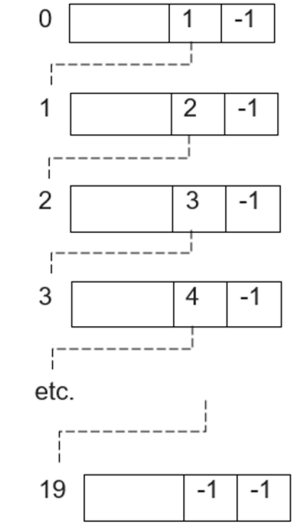
\includegraphics[width=0.15\paperwidth]{C:/Users/Admin/Desktop/Github/question_bank/LyX/static/img/9597-YIJC-2019-P1-Q3-1}
\par\end{center}

\subsection*{Task 3.1 }

Write a program code to define the \texttt{Node} and \texttt{ExpressionTree}
classes.

\subsection*{Evidence 3.1}

Your program code for Task 3.1. \hfill{}{[}12{]}

The task is to store the tokens of a binary arithmetic expression
in the data structure instantiated from the \texttt{ExpressionTree}
class. 

An arithmetic expression is a sequence of tokens that follows prescribed
rules. A token may be either an operand or an operator. 

A binary arithmetic operation using the standard arithmetic operators,
\texttt{+ - {*} /} , may be in the form of operand-operator-operand.
For example, 
\noindent \begin{center}
\texttt{2 + 3 }
\par\end{center}

where \texttt{2} and \texttt{3} are operands, \texttt{+} is an operator.
This expression will evaluate to a value of \texttt{5}. 

\subsection*{Task 3.2 }

Write a function \texttt{IsOperator(s)} that takes in a string \texttt{s},
and returns \texttt{True} if it is a standard arithmetic operator
and returns \texttt{False} if otherwise. 

\subsection*{Evidence 3.2 }

Your program code for Task 3.2. \hfill{}{[}2{]}

An expression tree is a binary tree with the following properties: 
\begin{enumerate}
\item[1.]  Each leaf is an \emph{operand}. 
\item[2.]  The root and internal nodes are \emph{operators}. 
\item[3.]  Subtrees are sub-expressions, with the root being an \emph{operator}.
\end{enumerate}
The following shows a series of commands to create and insert values
into the data structure to create an expression tree. 

\begin{minipage}[t]{0.5\columnwidth}%
\texttt{CreateNewExpTree }

\texttt{InsertToExpTree(\textquotedbl +\textquotedbl ) }

\texttt{InsertToExpTree(\textquotedbl{*}\textquotedbl ) }

\texttt{InsertToExpTree(\textquotedbl 4\textquotedbl ) }

\texttt{InsertToExpTree(\textquotedbl 2\textquotedbl ) }

\texttt{InsertToExpTree(\textquotedbl /\textquotedbl ) }

\texttt{InsertToExpTree(\textquotedbl 3\textquotedbl )}

\texttt{InsertToExpTree(\textquotedbl 1\textquotedbl )}%
\end{minipage}

The figure below shows the expression tree obtained and its \textbf{infix}
expression obtained by an in-order traversal. 

This expression will evaluate to \texttt{10}.
\begin{center}
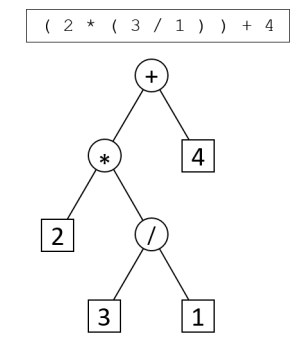
\includegraphics[width=0.25\paperwidth]{C:/Users/Admin/Desktop/Github/question_bank/LyX/static/img/9597-YIJC-2019-P1-Q3-2}
\par\end{center}

The following pseudocode (available in \texttt{PSEUDOCODE\_TASK\_3\_3.TXT})
can be used to add a node to the expression tree. 

\begin{minipage}[t]{0.88\columnwidth}%
\texttt{PROCEDURE Insert(NewToken)}

\texttt{\qquad{}IF NextFreeChild = -1 THEN // check if tree is full }

\texttt{\qquad{}\qquad{}RETURN 'Tree is Full'}

\texttt{\qquad{}// tree is not full, safe to insert new token }

\texttt{\qquad{}IF NextFreeChild = 0 THEN // inserting into empty
Tree }

\texttt{\qquad{}\qquad{}Tree{[}Root{]}.DataValue NewToken }

\texttt{\qquad{}\qquad{}NextFreeChild }

\texttt{\qquad{}\qquad{}Tree{[}Root{]}.LeftChild Tree{[}Root{]}.LeftChild
-1}

\texttt{\qquad{}ELSE }

\texttt{\qquad{}\qquad{}// inserting into tree with existing }

\texttt{\qquad{}\qquad{}// starting with Root }

\texttt{\qquad{}\qquad{}Current 0 // index of the current node }

\texttt{\qquad{}\qquad{}Previous -1 // index of previous node }

\texttt{\qquad{}\qquad{}NewNode Tree{[}NextFreeChild{]} // declare
new node }

\texttt{\qquad{}\qquad{}NewNode.DataValue NewToken }

\texttt{\qquad{}\qquad{}\qquad{}// Finding the node at which the
NewNode can be inserted }

\texttt{\qquad{}\qquad{}\qquad{}WHILE Current <> -1 THEN }

\texttt{\qquad{}\qquad{}\qquad{}\qquad{}CurrNode Tree{[}Current{]} }

\texttt{\qquad{}\qquad{}\qquad{}IF IsOperator(CurrNode.DataValue)
THEN }

\texttt{\qquad{}\qquad{}\qquad{}// check if CurrNode contains an
operator }

\texttt{\qquad{}\qquad{}\qquad{}\qquad{}IF CurrNode.LeftChild
= -1 THEN }

\texttt{\qquad{}\qquad{}\qquad{}\qquad{}// if LeftChild is empty,
insert here }

\texttt{\qquad{}\qquad{}\qquad{}\qquad{}\qquad{}CurrNode.LeftChild
NextFreeChild }

\texttt{\qquad{}\qquad{}\qquad{}\qquad{}\qquad{}NextFreeChild
NewNode.LeftChild }

\texttt{\qquad{}\qquad{}\qquad{}\qquad{}\qquad{}NewNode.LeftChild
-1 }

\texttt{\qquad{}\qquad{}\qquad{}\qquad{}\qquad{}Current -1}

\texttt{\qquad{}\qquad{}\qquad{}\qquad{}ELIF CurrNode.RightChild
= -1 THEN}

\texttt{\qquad{}\qquad{}\qquad{}\qquad{}\qquad{}// if RightChild
is empty, insert here }

\texttt{\qquad{}\qquad{}\qquad{}\qquad{}\qquad{}CurrNode.RightChild }

\texttt{\qquad{}\qquad{}\qquad{}\qquad{}\qquad{}NextFreeChild
NextFreeChild \textleftarrow{} NewNode.LeftChild }

\texttt{\qquad{}\qquad{}\qquad{}\qquad{}\qquad{}NewNode.LeftChild
-1}

\texttt{\qquad{}\qquad{}\qquad{}\qquad{}\qquad{}Current -1 }

\texttt{\qquad{}\qquad{}\qquad{}\qquad{}ELIF IsOperator(Tree{[}CurrNode.LeftChild{]}.DataValue)
THEN }

\texttt{\qquad{}\qquad{}\qquad{}\qquad{}\qquad{}// if LeftChild
is an operator, }

\texttt{\qquad{}\qquad{}\qquad{}\qquad{}\qquad{}// traverse leftchild
subtree }

\texttt{\qquad{}\qquad{}\qquad{}\qquad{}\qquad{}Previous Current }

\texttt{\qquad{}\qquad{}\qquad{}\qquad{}\qquad{}Current CurrNode.LeftChild}

\texttt{\qquad{}\qquad{}\qquad{}\qquad{}\qquad{}Fringe.APPEND(Previous)}

\texttt{\qquad{}\qquad{}\qquad{}\qquad{}ELIF IsOperator(Tree{[}CurrNode.RightChild{]}.DataValue)THEN }

\texttt{\qquad{}\qquad{}\qquad{}\qquad{}\qquad{}// if RightChild
is an operator, }

\texttt{\qquad{}\qquad{}\qquad{}\qquad{}\qquad{}// traverse rightchild
subtree }

\texttt{\qquad{}\qquad{}\qquad{}\qquad{}\qquad{}Previous Current}

\texttt{\qquad{}\qquad{}\qquad{}\qquad{}\qquad{}Current CurrNode.RightChild }

\texttt{\qquad{}\qquad{}\qquad{}\qquad{}\qquad{}Fringe.APPEND(Previous) }

\texttt{\qquad{}\qquad{}\qquad{}\qquad{}ELSE // traverse right
subtree }

\texttt{\qquad{}\qquad{}\qquad{}\qquad{}\qquad{}Previous Fringe.POP(-1) }

\texttt{\qquad{}\qquad{}\qquad{}\qquad{}\qquad{}Current Tree{[}Previous{]}.RightChild}

\texttt{\qquad{}\qquad{}\qquad{}\qquad{}ENDIF }

\texttt{\qquad{}\qquad{}\qquad{}ELSE // no place to insert}

\texttt{\qquad{}\qquad{}\qquad{}\qquad{}RETURN \textquotedbl Cannot
be inserted\textquotedbl{} }

\texttt{\qquad{}\qquad{}\qquad{}ENDIF }

\texttt{\qquad{}\qquad{}ENDWHILE}

\texttt{\qquad{}ENDIF}

\texttt{ENDPROCEDURE}%
\end{minipage}

\subsection*{Task 3.3 }

Write a code to implement the \texttt{Insert} method for the \texttt{ExpressionTree}
class from this pseudocode.

You may use the text file \texttt{PSEUDOCODE\_TASK\_3\_3.TXT} as a
basis for writing your code.

\subsection*{Evidence 3.3 }

Your program code for Task 3.3. \hfill{}{[}7{]}

\subsection*{Task 3.4: }

Write a code for the \texttt{Display} method for the \texttt{ExpressionTree}
class which displays the contents of \texttt{Tree} in index order. 

\subsection*{Evidence 3.4 }

Your program code for Task 3.4. \hfill{} {[}4{]}

\subsection*{Task 3.5 }

Write a sequence of program statements to: 
\begin{itemize}
\item create an expression tree
\item add the data items based on the sequence of commands given 
\item display the array contents 
\end{itemize}

\subsection*{Evidence 3.5 }

Your program code for Task 3.5. \hfill{}{[}3{]}

\subsection*{Evidence 3.6 }

Screenshot showing the output from running the program in Task 3.5.
\hfill{}{[}1{]}

\subsection*{Task 3.6 }

The infix notation can be obtained by performing an in-order traversal
in the expression tree. 

Write a code for the \texttt{infix} method for the \texttt{ExpressionTree}
class to generate the infix notation for a complete expression tree. 

\subsection*{Evidence 3.7 }

Your program code for Task 3.6. \hfill{} {[}6{]}

\subsection*{Evidence 3.8 }

Screenshot showing the output from running the program in Task 3.6.
\hfill{} {[}1{]}

\subsection*{Task 3.7 }

Write a code for the \texttt{calculate} method to evaluate and return
the numerical answer for the expression, rounded off to 2 decimal
places. 

\subsection*{Evidence 3.9 }

Your program code for Task 3.7. \hfill{}{[}3{]}

\subsection*{Evidence 3.10 }

Screenshot showing the output from running the program in Task 3.7.
\hfill{}{[}1{]}

{[}SPLIT\_HERE{]}
\item \textbf{{[}YIJC/PRELIM/9597/2019/P1/Q4{]} }

Minesweeper is a type of single-player puzzle game in which the player
continuously selects a cell in a square grid. Each cell contains either
a bomb or a value showing the number of bombs in the neighbouring
cell. (Neighbouring cells are those adjacent horizontally, vertically
or diagonally.)

If the player selects a cell that is a bomb, it \textquoteleft explodes\textquoteright{}
and he loses the game. The number of cells the player has selected
without exploding a bomb will be the player\textquoteright s score.

You are required to write a program code to generate a minesweeper
grid, randomly position the bombs and populate all the other cells
with the values indicating the number of bombs in the neighbouring
cells. Without revealing the minesweeper grid to the player, the program
should prompt the player to select the cells one by one. His score
will be the number of cells opened before hitting a bomb. 
\noindent \begin{center}
\begin{minipage}[t]{0.25\columnwidth}%
\texttt{X 2 1 1 }

\texttt{1 3 X 2 }

\texttt{0 2 X 3 }

\texttt{0 1 2 X }%
\end{minipage}
\par\end{center}

\subsection*{Task 4.1: }

Write a program code to generate and display an empty square grid
of size $n$, ie $n$ rows by $n$ columns. The minesweeper grid for
$n=5$ is as shown below: 
\noindent \begin{center}
\begin{minipage}[t]{0.25\columnwidth}%
\texttt{0 0 0 0 0 }

\texttt{0 0 0 0 0 }

\texttt{0 0 0 0 0 }

\texttt{0 0 0 0 0}

\texttt{0 0 0 0 0 }%
\end{minipage}
\par\end{center}

Your code should use a suitable data structure and fixed loop(s) to
display the grid.

\subsection*{Evidence 4.1: }

Your program code and screenshot of an empty grid of size 5.\hfill{}
{[}3{]}


\subsection*{Task 4.2: }

Write a program code to randomly place a bomb, represented by \textquotedbl X\textquotedbl ,
within the grid. Populate all the neighbouring cells by increasing
their values to 1 to indicate the presence of this one bomb in the
neighbourhood. 

\subsection*{Evidence 4.2: }

Your program code and two different screenshots of the grid ($n=5$).
\hfill{}{[}5{]}

\subsection*{Task 4.3: }

Modify the code written in Task 4.2 to randomly place two bombs within
the grid. Populate all the neighbouring cells with the correct values
to indicate the presence of the bombs in the neighbourhood. 

\subsection*{Evidence 4.3: }

Your program code and the screenshot of the grid ($n=5$) with 2 bombs.\hfill{}
{[}4{]}

\subsection*{Task 4.4: }

Modify the code written in Task 4.3 to generate $k$ numbers of bombs
within a grid of size $n$ and correctly display all the values in
the neighbouring cells surrounding the bombs. 

\subsection*{Evidence 4.4: }

Your program code and the screenshots of the minesweeper grids for
the following levels of difficulty. 
\begin{itemize}
\item Beginner (grid size $n=5$; no. of bombs $k=3$)
\item Intermediate (grid size $n=6$; no. of bombs $k=8$)
\item Expert (grid size $n=8$; no. of bombs $k=20$) {[}8{]}
\end{itemize}

\subsection*{Task 4.5: }

Write a program code to play the minesweeper game. Your code will:
\begin{itemize}
\item prompt the player to select the level of difficulty
\item generate the Minesweeper grid 
\item display a \textquotedblleft blank\textquotedblright{} grid with \textquoteleft -\textquoteright{}
for each of the cell prompt the player to input the coordinates of
a cell he wishes to open 
\begin{itemize}
\item If the opened cell is a bomb (\textquotedblleft X\textquotedblright ),
declare \textquotedblleft Game Over!\textquotedblright , show the
grid and display the player\textquoteright s score.
\item If the opened cell is not a bomb, show the updated grid with the opened
cell, increase the player\textquoteright s score by 1 and continue
with the game.
\end{itemize}
\item declare \textquotedblleft You have Won!\textquotedblright{} when the
player has opened all the possible cells and display the player\textquoteright s
score. 

{[}Sample screenshot of a typical game{]}: 

\noindent %
\begin{minipage}[t]{0.5\columnwidth}%
\texttt{Enter your cell you want to open:}

\texttt{X (1 to 5) : 2}

\texttt{Y (1 to 5) : 3}

\texttt{\_ \_ \_ \_ \_}

\texttt{\_ \_ 1 \_ \_}

\texttt{0 \_ \_ \_ \_}

\texttt{\_ \_ 1 \_ \_}

\texttt{\_ \_ \_ \_ \_}

\texttt{Your score is : 3}%
\end{minipage}%
\begin{minipage}[t]{0.5\columnwidth}%
\texttt{Enter your cell you want to open:}

\texttt{X (1 to 5) : 2}

\texttt{Y (1 to 5) : 4}

\texttt{X 1 1 1 1}

\texttt{1 1 1 X 1}

\texttt{0 0 1 1 1}

\texttt{0 1 1 1 0}

\texttt{0 1 X 1 0}

\texttt{Game over! You've hit the bomb at : (2,4).}

\texttt{Your score is : 3}

\texttt{Do you want to try again?}%
\end{minipage}
\end{itemize}

\subsection*{Evidence 4.5:}

Your program code and a screenshot of a game. \hfill{}{[}10{]}

{[}SPLIT\_HERE{]}
\end{enumerate}

\end{document}
